%-----------------------------------------------------
% index key words
%-----------------------------------------------------
\index{dot product}
\index{angle between vectors}

%-----------------------------------------------------
% name, leave blank
% title, if the exercise has a name i.e. Hilbert's matrix
% difficulty = n, where n is the number of stars
% origin = "\cite{ref}"
%-----------------------------------------------------
\begin{Exercise}[
name={},
title={}, 
difficulty=0,
origin={\cite{MH}}]
Suppose that $\vec u$ and $\vec v$ are two vectors in the $xy$-plane with directions as given in the diagram and such that $\vec u$ has length 2 and $\vec v$ has length 3.
\begin{minipage}[m]{\linewidth}
\centering
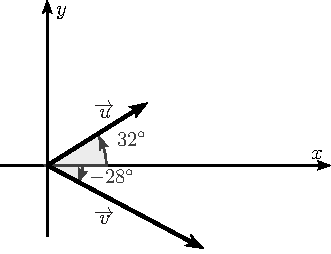
\includegraphics[width=\linewidth/2]{vector_geometry/dot_product_and_projections/figures/mh2}
\end{minipage}
\Question Find $\vec u\cdot\vec v$.
\Question Find $\norm{\vec u+\vec v}$.
\end{Exercise}

\begin{Answer}


\end{Answer}
